\section{Signal Path}
\label{signPath}

The simulated path that the \ac{laser} signal follows is visualized in figure \ref{signPath} on 
page \pageref{signPath}. There are three distinct phases. The first one is the downtravel of the
signal trough the atmosphere. This is followed by the reflection on the Earth's surface. Finally the
pulse has to travel back up through the atmosphere. This sequence is elaborated below in more
detail.

The signal originates from the emitter. The for each pulse, the emitter position is determined from
a set of Kepler elements. The energy in the pulse is found by distributing the emitter power over a
constant number of pulses of a given duration.

The signal then starts to propagate through the atmosphere. The atmosphere effects the signal in
several manners, but the most important one is the attenuation of the signal. Attenuation is the
only disturbance by the atmosphere taken into account. The pulse energy exponentially decays with
distance travel though the atmosphere. Furthermore also the optical thickness of the atmosphere is a
parameter in this process.

Then the intersection of the pulse with the \ac{DEM} is computed. As a simplification in this
process, the intersection of the pulse (ray) with a sphere is computed. The sphere has a radius of
the average terrain height of the \ac{DEM} tile plus the Earth radius. Then the ray-sphere
intersection point coordinates are covered into latitude and longitude. These are then used to 
find the actual terrain elevation from the \ac{DEM} and the 3D position.

Then the scattering characteristics are constructed. For this, the terrain normal and the inbound
laser pulse vector are utilized. The power of the emitted pulse is now distributed over the entire
footprint area off the emitter and then scattered back using the scattering technique described in
section \ref{scatter}. The backscattered energy is computed separately for every receiver satellite.

The reflected pulse now travels back trough 1the atmosphere. This causes more attenuation to take
place. The energy received by the receivers is now dependent on the receiver aperture. This received
energy can then converted into photons by dividing by the energy per photon.

\begin{figure}[ht!]
	\centering
		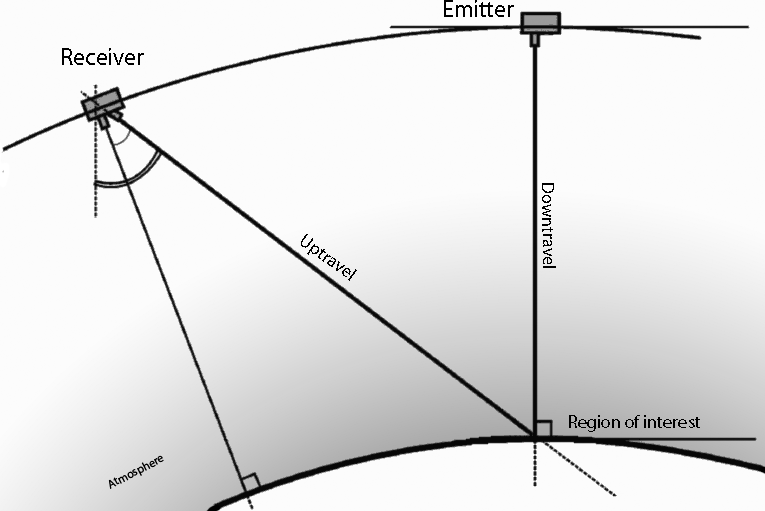
\includegraphics[width=0.8\textwidth]{chapters/img/signalPath.png}
		\label{fig:signalPath}
	\caption{Signal path representation}
\end{figure}










